\documentclass{standalone}
\usepackage{pgfplots}
\pgfplotsset{compat=newest}

\pagestyle{empty}

\begin{document}
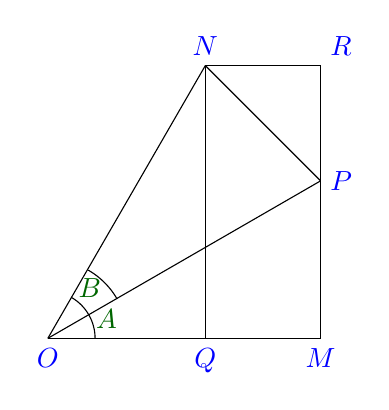
\begin{tikzpicture}
  \draw (0, 0) -- (3.464, 0);
  \draw (3.464, 0) -- (3.464, 2);
  \draw (0, 0) -- (3.464, 2);
  \draw (0, 0) -- (2, 0);
  \draw (2, 0) -- (2, 3.464);
  \draw (0, 0) -- (2, 3.464);
  \draw (2, 3.464) -- (3.464, 2);
  \draw (2, 3.464) -- (3.464, 3.464);
  \draw (3.464, 3.464) -- (3.464, 2);
  \draw (.6, 0) arc[start angle=0, end angle=60, radius=0.6];
  \draw (.88, .5) arc[start angle=30, end angle=60, radius=1];
  \draw [blue] (0, 0) node[anchor=north] {$O$};
  \draw [blue] (2, 0) node[anchor=north] {$Q$};
  \draw [blue] (3.464, 0) node[anchor=north] {$M$};
  \draw [blue] (3.464, 2) node[anchor=west] {$P$};
  \draw [blue] (3.464,3.464) node[anchor=south west] {$R$};
  \draw [blue] (2, 3.464) node[anchor=south] {$N$};
  \draw [black!60!green] (1, 0) node[anchor=south east] {$A$};
  \draw [black!60!green] (.8, .4) node[anchor=south east] {$B$};
\end{tikzpicture}
\end{document}
